\subsection{Ensemble: Random Forest}
 
\paragraph{Cây quyết định CART với tiêu chí Gini.} Mỗi nút trong hỏi một câu nhị phân ``$x_f\le t$?''; mẫu thoả điều kiện đi sang nhánh trái, còn lại sang phải. Độ vẩn đục Gini của một nút có tỉ lệ lớp $p_k$:
\begin{equation}
G=1-\sum_{k=1}^{K}p_k^2,
\end{equation}
bằng 0 khi nút thuần nhất và đạt tối đa $1-1/K$ khi các lớp chia đều. Với $n$ mẫu tại nút, $n_L$, $n_R$ mẫu ở hai nhánh, phép tách $(f,t)$ được chọn để \emph{độ giảm Gini} lớn nhất:
\begin{equation}
\Delta(f,t)=G_{\text{cha}}-\underbrace{\Big(\tfrac{n_L}{n}G_L+\tfrac{n_R}{n}G_R\Big)}_{\text{Gini có trọng số}}.
\end{equation}
Trọng số $n_L/n$, $n_R/n$ ngăn thuật toán ưa các phép tách ``cắt riêng một mẫu'' (nhánh nhỏ thuần nhưng nhánh lớn vẫn hỗn loạn). Cây phát triển đệ quy tới khi gặp điều kiện dừng; mỗi lá lưu vector tỉ lệ lớp $\mathbf{p}_{\text{lá}}\in\R^K$.
 
\paragraph{Hai nguồn ngẫu nhiên và gộp kết quả.} Random Forest huấn luyện $T$ cây, mỗi cây $b$:
\begin{itemize}
\item học trên một mẫu \textbf{bootstrap} $\mathcal{D}_b$ gồm $n$ mẫu lấy \emph{có hoàn lại}; xác suất một mẫu không được chọn là $(1-1/n)^n\to e^{-1}\approx0.368$;
\item tại \textbf{mỗi nút} chỉ xét $m$ đặc trưng chọn ngẫu nhiên không lặp, với $m=\lfloor\sqrt{D}\rfloor=28$.
\end{itemize}
Hai nguồn này giảm tương quan $\rho$ giữa các cây. Với $T$ cây có phương sai $\sigma^2$, phương sai của trung bình là $\rho\sigma^2+\frac{1-\rho}{T}\sigma^2$: tăng $T$ triệt tiêu số hạng thứ hai, còn giảm $\rho$ làm nhỏ số hạng thứ nhất. Dự đoán dùng \emph{soft voting}:
\begin{equation}
P(c\mid\mathbf{x})=\frac1T\sum_{b=1}^{T}\mathbf{p}^{(b)}_{\text{lá}(\mathbf{x})}[c],\qquad \hat y=\argmax_c P(c\mid\mathbf{x}).
\end{equation}
 
\paragraph{OOB score và độ quan trọng đặc trưng.} Mẫu không nằm trong $\mathcal{D}_b$ là mẫu \emph{out-of-bag} (OOB) của cây $b$. Mỗi mẫu huấn luyện $i$ được dự đoán chỉ bởi các cây $\mathcal{B}_i=\{b: i\notin\mathcal{D}_b\}$, cho ước lượng accuracy trên dữ liệu chưa thấy mà không cần tập riêng:
\begin{equation}
\text{OOB}=\frac{1}{|\{i:\mathcal{B}_i\neq\varnothing\}|}\sum_{i:\mathcal{B}_i\neq\varnothing}\mathbb{1}\Big[\argmax_c\sum_{b\in\mathcal{B}_i}\mathbf{p}^{(b)}(\mathbf{x}_i)[c]=y_i\Big].
\end{equation}
Độ quan trọng của đặc trưng $f$ là tổng $n_{\text{nút}}\cdot\Delta$ qua mọi nút tách theo $f$, chuẩn hoá tổng bằng 1 trong từng cây, rồi lấy trung bình qua các cây.
 
\begin{algorithm}[H]
\caption{Tìm phép tách tốt nhất tại một nút (sắp xếp + tổng cộng dồn)}\label{alg:split}
\begin{algorithmic}[1]
\Function{BestSplit}{$X$, $\mathbf{y}$, tập đặc trưng $F$, $m_{\text{leaf}}$}
  \State $\Delta^*\gets0$;\; $\textit{best}\gets\varnothing$;\; $\mathbf{n}_L\gets(1,\dots,n-1)$;\; $\mathbf{n}_R\gets n-\mathbf{n}_L$
  \For{mỗi $f\in F$}
    \State sắp xếp mẫu theo $x_f$ tăng dần $\to$ $\mathbf{x}^s$, $\mathbf{y}^s$
    \State $H\gets\mathrm{onehot}(\mathbf{y}^s)\in\{0,1\}^{n\times K}$
    \State $C_L\gets\mathrm{cumsum}(H)$ bỏ hàng cuối;\; $C_R\gets\sum H-C_L$ \Comment{số mẫu mỗi lớp hai bên, mọi vị trí}
    \State $\mathbf{g}\gets\big(\mathbf{n}_L\,G(C_L/\mathbf{n}_L)+\mathbf{n}_R\,G(C_R/\mathbf{n}_R)\big)/n$ \Comment{Gini có trọng số, $n-1$ giá trị}
    \State $\textit{valid}_j\gets(x^s_j<x^s_{j+1})\wedge(n_{L,j}\ge m_{\text{leaf}})\wedge(n_{R,j}\ge m_{\text{leaf}})$
    \If{không có $j$ hợp lệ} \textbf{tiếp tục} với $f$ kế tiếp \EndIf
    \State $j^*\gets\argmin_{j\,\text{hợp lệ}}g_j$;\; $\Delta\gets G_{\text{cha}}-g_{j^*}$
    \If{$\Delta>\Delta^*$} $\Delta^*\gets\Delta$;\; $\textit{best}\gets\big(f,\;(x^s_{j^*}+x^s_{j^*+1})/2,\;\Delta\big)$ \EndIf
  \EndFor
  \State \Return \textit{best}
\EndFunction
\end{algorithmic}
\end{algorithm}
 
\begin{algorithm}[H]
\caption{Huấn luyện và dự đoán Random Forest}\label{alg:rf}
\begin{algorithmic}[1]
\Function{Grow}{$X$, $\mathbf{y}$, độ sâu $d$}
  \If{$d\ge d_{\max}$ \textbf{hoặc} $n<m_{\text{split}}$ \textbf{hoặc} $G(\mathbf{y})=0$} \Return Lá$(\text{tỉ lệ lớp của }\mathbf{y})$ \EndIf
  \State $F\gets m$ đặc trưng chọn ngẫu nhiên không lặp
  \State $(f,t,\Delta)\gets$ \Call{BestSplit}{$X,\mathbf{y},F,m_{\text{leaf}}$}
  \If{không tìm được} \Return Lá$(\text{tỉ lệ lớp của }\mathbf{y})$ \EndIf
  \State $\textit{imp}[f]\mathrel{+}=n\cdot\Delta$;\; $M\gets(X_{:,f}\le t)$
  \State \Return Nút$\big(f,t,$ \Call{Grow}{$X_M,\mathbf{y}_M,d{+}1$}, \Call{Grow}{$X_{\neg M},\mathbf{y}_{\neg M},d{+}1$}$\big)$
\EndFunction
\Function{FitForest}{$X$, $\mathbf{y}$, $T$}
  \State mã hoá nhãn về $0..K{-}1$; khởi tạo $\textit{oob\_sum}\in\R^{n\times K}$, $\textit{oob\_cnt}\in\R^n$ bằng 0
  \For{$b=1,\dots,T$}
    \State $\textit{rng}_b\gets$ bộ sinh ngẫu nhiên với hạt giống rút từ \code{random\_state}
    \State $I_b\gets n$ chỉ số ngẫu nhiên có hoàn lại trong $\{0,\dots,n{-}1\}$ \Comment{bootstrap}
    \State $\text{cây}_b\gets$ \Call{Grow}{$X_{I_b},\mathbf{y}_{I_b},0$}
    \State $O\gets\{i\notin I_b\}$;\; $\textit{oob\_sum}[O]\mathrel{+}=\text{cây}_b.\text{proba}(X_O)$;\; $\textit{oob\_cnt}[O]\mathrel{+}=1$
  \EndFor
  \State OOB $\gets$ tỉ lệ $\argmax\textit{oob\_sum}[i]=y_i$ trên các $i$ có $\textit{oob\_cnt}[i]>0$
\EndFunction
\Function{Predict}{$\mathbf{x}$}
  \State \Return $\argmax_c \frac1T\sum_b \text{cây}_b.\text{proba}(\mathbf{x})[c]$ \Comment{mỗi cây: đi từ gốc xuống lá}
\EndFunction
\end{algorithmic}
\end{algorithm}
 
\paragraph{Chi tiết cài đặt} (\code{random\_forest.py}, chỉ dùng NumPy).
\begin{itemize}
\item \textbf{Tìm ngưỡng chính xác, không chia bin.} Cách ngây thơ thử từng ngưỡng và đếm lại tốn $O(n^2)$ mỗi đặc trưng. Thuật toán~\ref{alg:split} sắp xếp một lần ($O(n\log n)$), mã hoá one-hot để biến ``đếm'' thành ``cộng'', rồi dùng \code{np.cumsum} để có số đếm lớp bên trái cho \emph{mọi} vị trí tách trong một lượt; bên phải bằng tổng trừ bên trái. Gini của cả $n-1$ vị trí được tính vector hoá nhờ broadcasting (\code{n\_left[:, None]}).
\item \textbf{Vị trí tách hợp lệ.} Điều kiện \code{xs[:-1] < xs[1:]} loại các vị trí nằm giữa hai giá trị bằng nhau (không ngưỡng nào tách được chúng, rất thường gặp vì nhiều pixel bằng 0); các vị trí không hợp lệ được gán $+\infty$ bằng \code{np.where} trước khi lấy \code{argmin}. Ngưỡng là trung điểm hai giá trị kề nhau. Đặc trưng không có vị trí hợp lệ (pixel hằng) bị bỏ qua; nếu không đặc trưng nào tách được, nút thành lá.
\item \textbf{Mã hoá nhãn và số lớp cố định.} \code{np.unique(y, return\_inverse=True)} đưa nhãn về $0..K{-}1$; $K$ được tính một lần ở rừng và truyền cho mọi cây, nên vector xác suất của mọi lá đều dài $K$ kể cả khi mẫu bootstrap thiếu lớp. \code{classes\_} dùng để đổi ngược về nhãn gốc khi dự đoán.
\item \textbf{Tái lập được.} Mỗi cây có bộ sinh riêng \code{default\_rng(rng.integers(2**31))} rút từ bộ sinh gốc \code{random\_state}; cùng hạt giống cho cùng một rừng.
\item \textbf{Hiệu năng.} Lớp \code{Node} dùng \code{\_\_slots\_\_} để giảm bộ nhớ; duyệt cây khi dự đoán bằng vòng \code{while} (không đệ quy). \code{max\_features} chấp nhận \code{"sqrt"}, \code{"log2"}, số thực (tỉ lệ) hoặc số nguyên và được quy về số nguyên bằng \code{\_resolve\_max\_features}; \code{voting} chọn \code{"soft"} hoặc \code{"hard"}. Dự đoán dùng vòng lặp Python theo từng ảnh nên chậm hơn các mô hình còn lại (khoảng 0.2\,ms/ảnh với 50 cây).
\end{itemize}
 
\paragraph{Cách kiểm chứng.}
\begin{enumerate}
\item \textbf{Tính tay.} Trên ví dụ 10 ảnh một đặc trưng (độ sáng pixel tâm, nhãn $0,0,0,0,1,1,7,1,7,7$), $G_{\text{cha}}=0.66$; in \code{child\_gini} của cả 9 vị trí tách và so với bảng tính tay: ngưỡng $t=0.40$ cho Gini có trọng số $0.300$, $\Delta=0.360$ lớn nhất; các ngưỡng $0.10$, $0.75$, $0.875$ cho $0.525$, $0.417$, $0.475$, khớp hoàn toàn.
\item \textbf{Dữ liệu tổng hợp có đáp án biết trước.} 3 lớp, 2 đặc trưng có ích và 6 đặc trưng nhiễu: rừng cho feature importance $\approx0.30$ và $0.34$ cho hai đặc trưng có ích, $\approx0.06$ cho mỗi đặc trưng nhiễu; accuracy rừng (0.849) vượt một cây (0.782).
\item \textbf{Đối chiếu scikit-learn}: so với lớp \code{RandomForestClassifier} dùng cùng \code{n\_estimators}, \code{max\_depth}, \code{min\_samples\_leaf} và \code{max\_features} $=\sqrt{D}$. Vì có ngẫu nhiên, tiêu chí là accuracy gần nhau chứ không phải trùng từng dự đoán (Bảng~\ref{tab:sklearn}).
\item \textbf{Nhất quán nội tại.} OOB score phải gần accuracy validation, và bản đồ importance phải bằng 0 ở các pixel viền luôn tối. Kết quả: OOB $=0.9549$ so với val $0.9622$ (thấp hơn khoảng 0.7 điểm, đúng kỳ vọng vì mỗi mẫu OOB chỉ được khoảng 37\% số cây bỏ phiếu); 158/784 pixel không bao giờ được dùng để tách (bao gồm 67 pixel luôn bằng 0), và importance tập trung ở vùng tâm nơi các nét chữ phân biệt nhau (Hình~\ref{fig:rf_importance}).
\end{enumerate}
 
\begin{figure}[H]
\centering
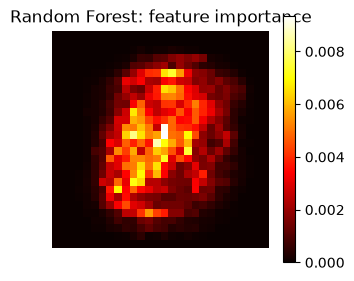
\includegraphics[width=0.4\textwidth]{figures/rf_importance.png}
\caption{Feature importance của Random Forest (50 cây) vẽ thành ảnh $28\times28$.}\label{fig:rf_importance}
\end{figure}